\subsection{Case03 - Echo server}
\label{xdp_wifi_case03}

En este caso de uso se explorará el análisis de paquetes, su filtrado y manejo. En los anteriores caso de uso exclusivamente se definía un comportamiento de los paquetes haciendo un uso exclusivo de los códigos de retorno \gls{xdp}, más concretamente \texttt{XDP\_DROP} para tirar los paquetes y \texttt{XDP\_PASS} para admitir los paquetes.\\
\par
Por tanto, en este test se filtrarán los paquetes por sus cabeceras, haciendo uso de las estructuras indicadas en este mismo caso de uso en un entorno cableado (Ir a \ref{xdp_ether_case03}). Se filtrarán los paquetes ICMP con el código \texttt{ECHO-Request}, se modificarán sus campos para conformar su respuesta, y se reenviará dicho paquete a la misma interfaz por la cual llegó para que sea entregado a su emisor. De esta forma se conformará un servidor de Echo, que responderá a todos los pings que lleguen a la interfaz que tenga cargado este programa \gls{xdp}. 

\vspace{0.5cm}
\textbf{Compilación}\\
\par

Para compilar el programa \gls{xdp}, al igual que en casos de uso anteriores, se ha dejado un Makefile preparado en este directorio. Por lo tanto, para compilarlo únicamente hay que seguir las indicaciones del bloque \ref{code:case03_xdp_wifi_compilacion}.

\begin{lstlisting}[language= bash, style=Consola, caption={Compilación programa XDP - Case03},label=code:case03_xdp_wifi_compilacion]
    # En caso de no haber entrado en el directorio asignado del caso de uso
    cd TFG/src/use_cases/xdp-wireless/case03
    
    
    # Hacemos uso del Makefile suministrado 
    sudo make
\end{lstlisting}
\vspace{0.5cm}

Si tiene dudas sobre el proceso de compilación del programa \gls{xdp} le recomendamos que vuelva al case02 (\gls{xdp} - Cableado \ref{xdp_ether_case02}) donde se hace referencia al \textit{flow} dispuesto para la compilación de los programas \gls{xdp}.\\
\par



\vspace{0.5cm}
\textbf{Puesta en marcha del escenario}\\
\par

Para testear los programas \gls{xdp} en un entorno inalámbrico, se hará uso de Mininet-WiFi para emular las topologías de red. Para levantar el escenario solo se tendrá que ejecutar el script en Python que hace uso de la API de Mininet-WiFi para generar toda la topología de red. Una vez ejecutado este abrirá la interfaz de linea de comandos de Mininet-WiFi, desde la cual se podrá comprobar el funcionamiento del caso de uso. En este caso, se realiza la carga del programa XDP desde el propio script de Python, haciendo uso de la herramienta xdp\_loader desarrollada para ello. \\
\par

Para limpiar la máquina del escenario recreado anteriormente con Mininet-WiFi se podría realizar un \texttt{sudo mn -c}, pero se recomienda al usuario que haga uso del \textit{target} del Makefile destinado para ello, ya que adicionalmente limpiará los ficheros intermedios generados en el proceso de compilación de nuestro programa \gls{xdp}. Ejecutando el siguiente comando se limpiaría la máquina.
\newpage
\begin{lstlisting}[language= bash, style=Consola, caption={Compilación programa XDP - Case03},label=code:case03_xdp_wifi_run]
    # Levantamos el escenario
    sudo python runenv.py
    
    
    # Limpiamos el escenario
    sudo make clean
\end{lstlisting}
\vspace{0.7cm}


Por último, únicamente indicar que el escenario recreado es el siguiente, compuesto exclusivamente de dos estaciones \textit{wireless}, aisladas en sus propias \textit{Network Namespaces}, y un punto de acceso corriendo el \textit{daemon} de HostApd para intercomunicar dichas estaciones WiFi.\\
\par

% figura escenario
\begin{figure}[ht]
    \centering
    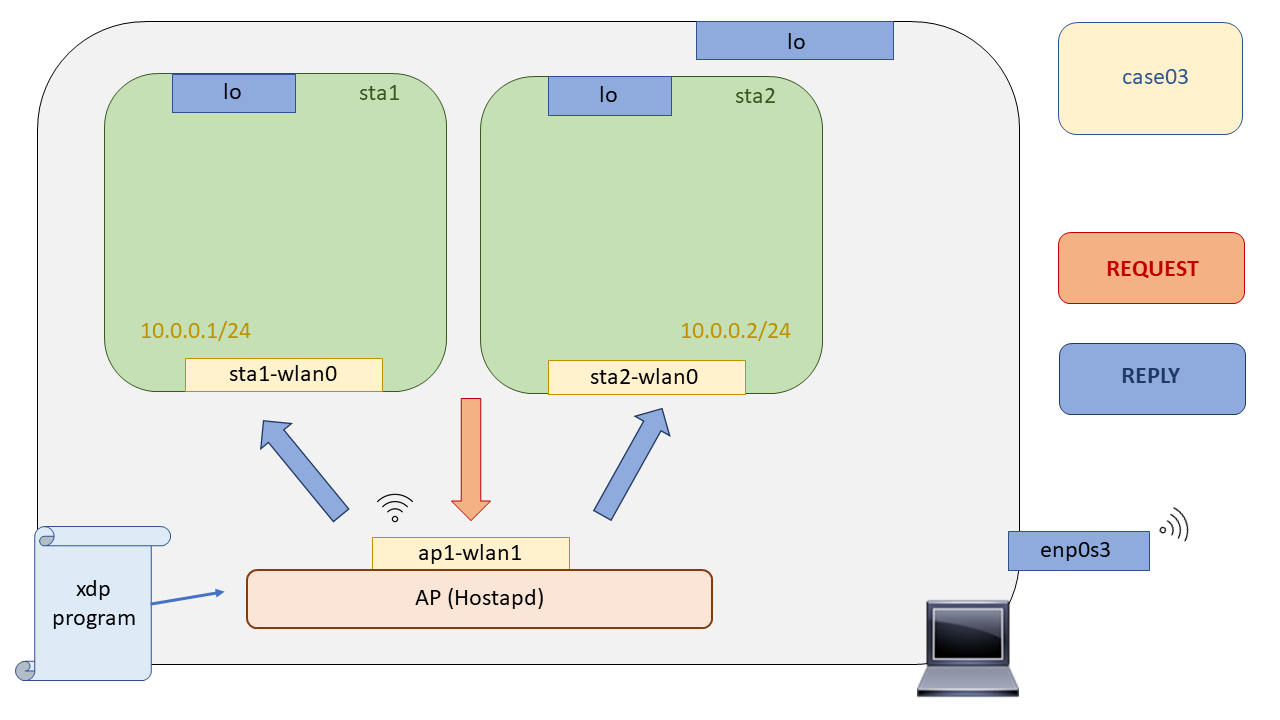
\includegraphics[width=16cm]{archivos/img/dev/xdp-wifi/case03/scenario.png}
    \caption{Escenario inalámbrico del Case03 - XDP}
    \label{fig:case03_xdp_wifi_scenario}
\end{figure}


\vspace{0.6cm}
\textbf{Carga del programa XDP}\\
\par
Como ya se ha comentado, la carga del programa \gls{xdp}, se llevará a cabo en el proceso del levantamiento del escenario, descrito en el script de Python para crear la topología. La carga del programa \gls{xdp}, se hará con el programa \texttt{xdp\_loader}, utilizado anteriormente para cargar los programas \gls{xdp} en interfaces alámbricas. 

\newpage

\begin{lstlisting}[language= bash, style=Consola, caption={Carga del programa XDP - Case03},label=code:case03_xdp_wifi_load]
    # Linea 37 del script runenv.py
    ap1.cmd("./xdp_loader -S -d ap1-wlan1 -F --progsec xdp_case03")
\end{lstlisting}
\vspace{0.5cm}
En este caso, se puede apreciar como la carga del programa \gls{xdp} se está llevando a cabo sobre la interfaz del punto de acceso \texttt{ap1}. Dado que únicamente son los paquetes ICMP los que serán interceptados y contestados, los paquetes de control del punto de acceso no se verán afectados, irán directamente al \textit{daemon} HostApd haciendo uso del código de retorno \texttt{XDP\_PASS}.\\
\par


\vspace{0.5cm}
\textbf{Comprobación del funcionamiento}\\
\par

La comprobación del funcionamiento del programa \gls{xdp} anclado a la interfaz \texttt{ap1-wlan1} se llevará a cabo generando pings desde las estaciones wireless hacia el punto de acceso, para que la interfaz \texttt{ap1-wlan1} los filtre, analice y nos genere una respuesta. Si todo funciona correctamente deberíamos ver como los códigos de retorno mayormente empleados son los de \texttt{XDP\_TX} siempre y cuando no hayamos detenido el ping desde dentro de la \textit{Network Namespace}. 


\begin{lstlisting}[language= bash, style=Consola, caption={Comprobación del funcionamiento - Case03},label=code:case03_xdp_wifi_func1]
    # Lanzamos un ping desde una estación wireless hacia cualquier máquina
    mininet-wifi> sta1 ping 9.9.9.9
    
    # En una consola aparte lanzamos el programa xdp_stats para ir viendo a tiempo real
    # los códigos de retorno XDP empleados
    mininet-wifi> ap1 ./xdp_stats -d ap1-wlan1
\end{lstlisting}

% figura escenario
\begin{figure}[ht!]
    \centering
    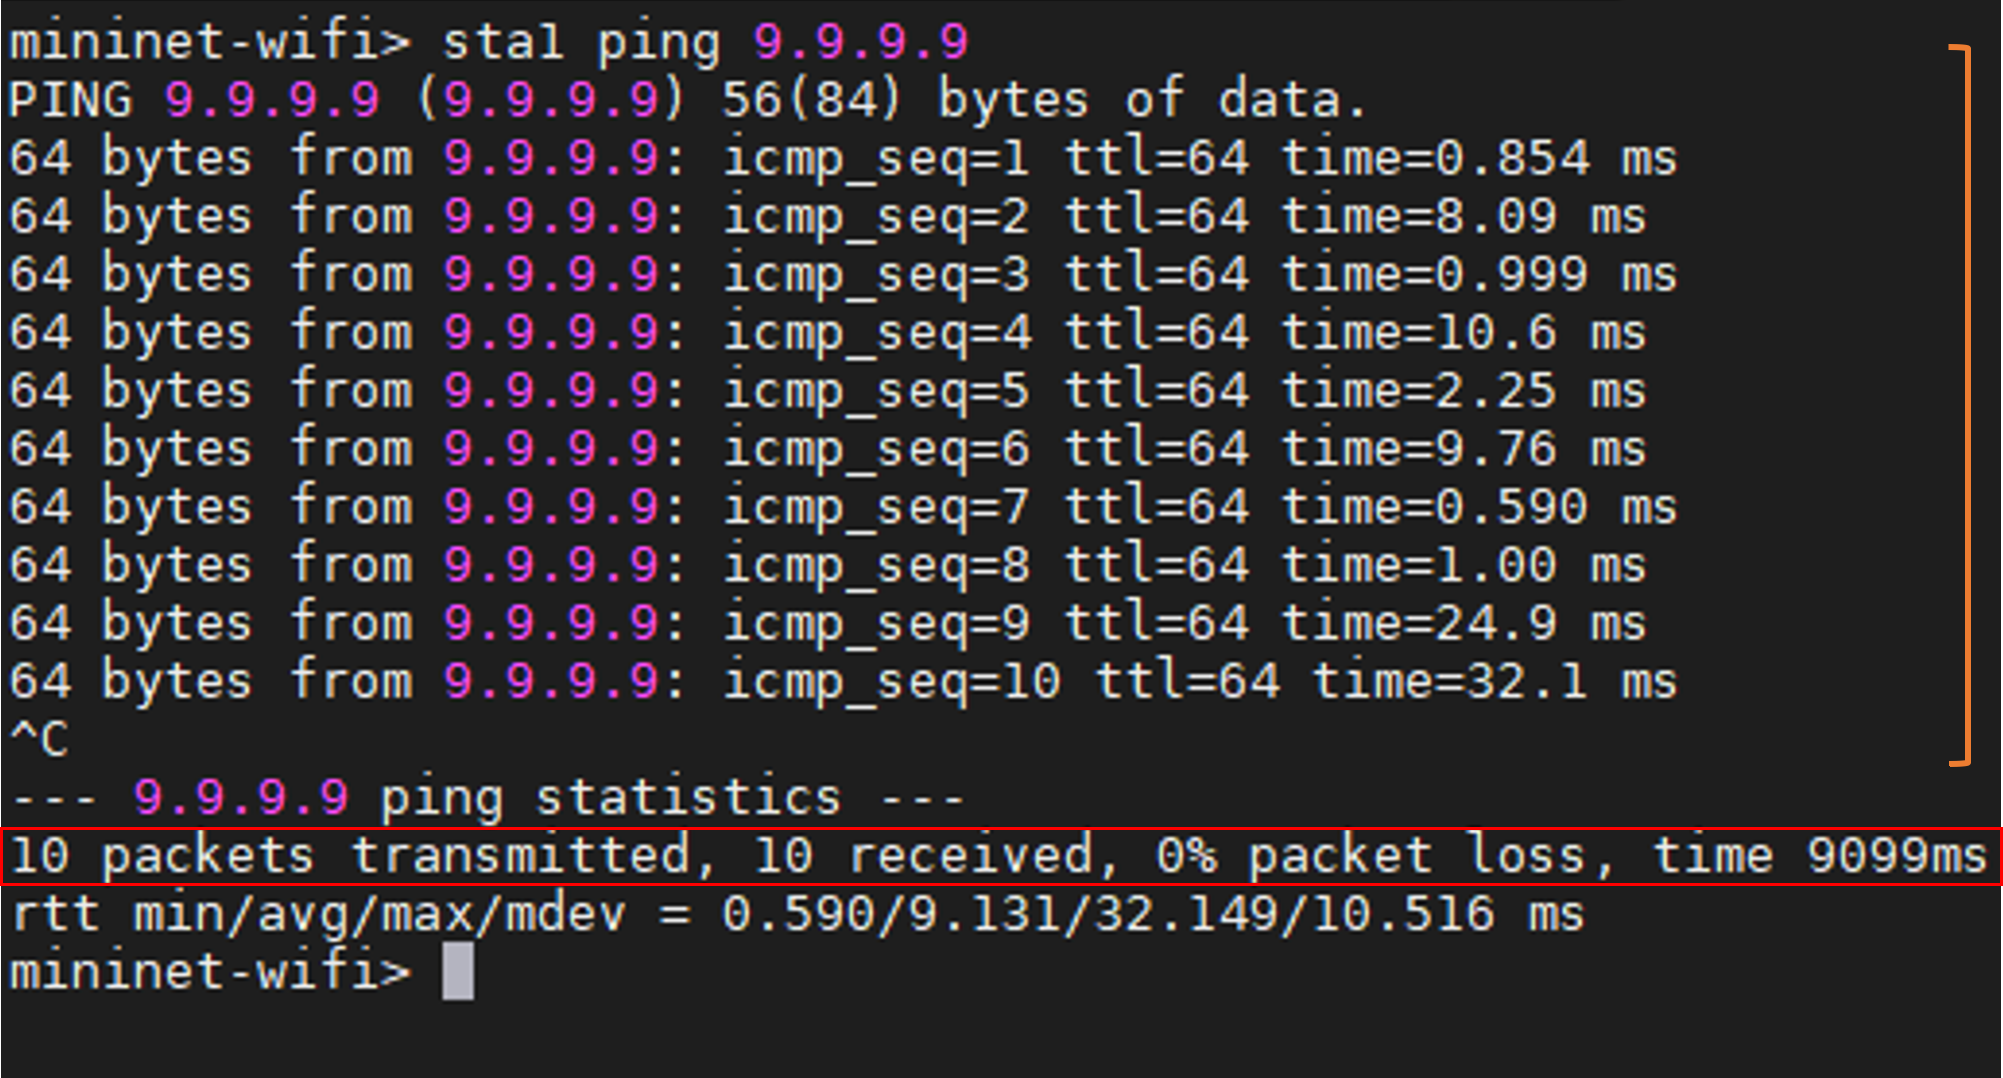
\includegraphics[width=12cm]{archivos/img/dev/xdp-wifi/case03/demo_case03_1_edited.png}
    \caption{Comprobación de funcionamiento (Ping) del Case03 - XDP Wireless}
    \label{fig:case03_xdp_wifi_func1}
\end{figure}

Como se puede ver en la figura \ref{fig:case03_xdp_wifi_func1}, se está realizando ping hacia una máquina inexistente, pero como en el script de aprovisionamiento se le han indicado a todas las estaciones WiFi un hipotético \textit{gateway}, y se ha añadido en la tabla ARP la MAC de ese hipotético \textit{gateway}, no habrá una resolución ARP previa al envío del ping. Por tanto se generará el ping \fcolorbox{black}{orange}{\rule{0pt}{2.5pt}\rule{2.5pt}{0pt}}\hspace{1mm}, que llegará a la interfaz la cual tiene cargado el programa \gls{xdp}, y como se puede apreciar en la figura \ref{fig:case03_xdp_wifi_func2}, dichos pings \fcolorbox{black}{orange}{\rule{0pt}{2.5pt}\rule{2.5pt}{0pt}}\hspace{1mm} son contestados correctamente por el programa devolviendo códigos de retorno \texttt{XDP\_TX}.

% figura escenario
\begin{figure}[ht!]
    \centering
    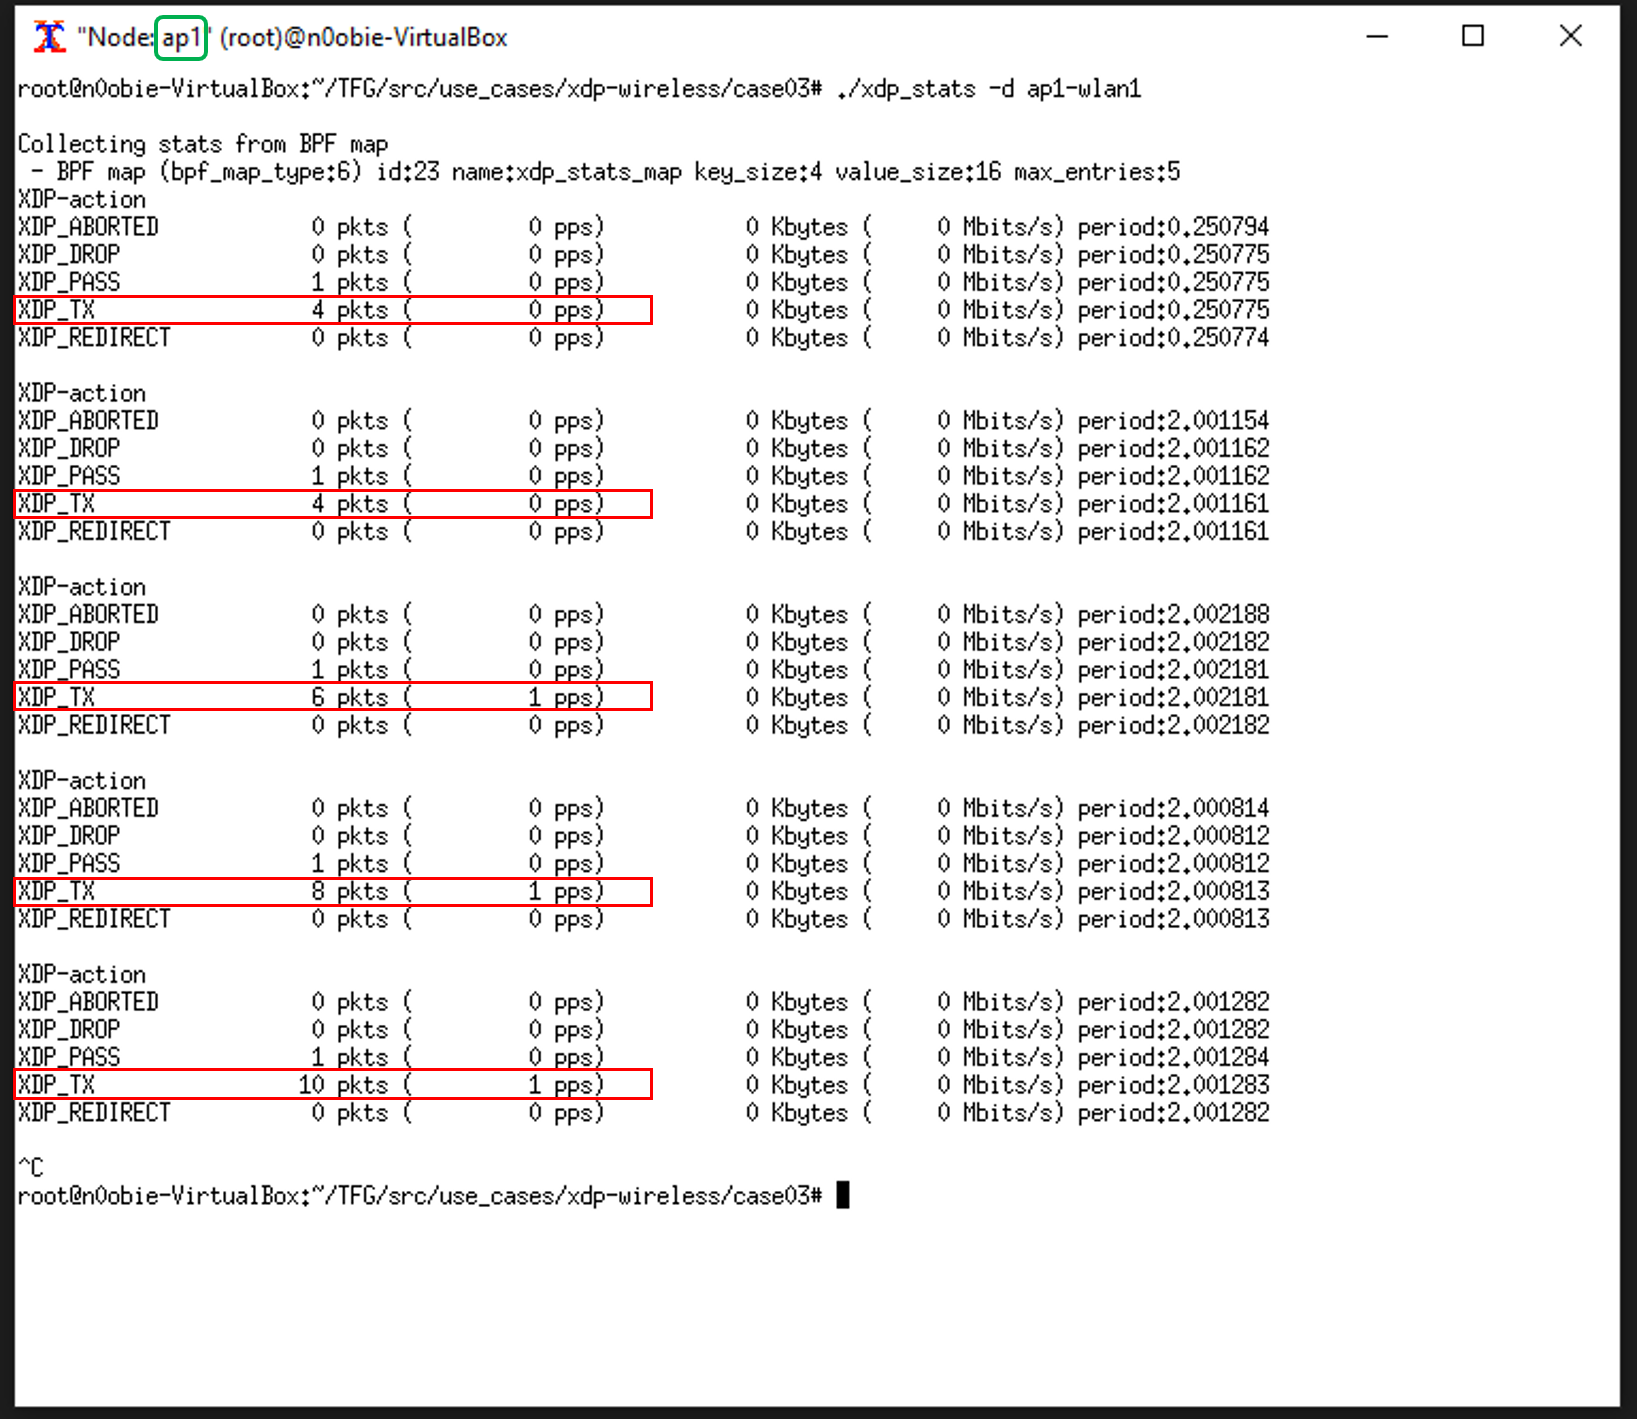
\includegraphics[width=15.5cm]{archivos/img/dev/xdp-wifi/case03/demo_case03_2_edited.png}
    \caption{Comprobación de funcionamiento (Stats) del Case03 - XDP Wireless}
    \label{fig:case03_xdp_wifi_func2}
\end{figure}

